\chapter{业务流程分析}

\section{概述}
系统的角色分为难民,房主,编辑者和管理员四个。其中难民可以登录也可以不登陆,不登陆只能浏览救助房源信息,但是不能进行举报,举报功能只针对登录用户。
后三个角色一定需要登录才能继续操作,房主除了登录之外还需要进行身份认证,作为自己提供的房源提供保障,也方便系统做后续的追踪工作。管理员和编辑员的账号是已经在系统中预定义的,直接登录即可。
管理员的权限最高,能够对所有用户进行管理,能够拥有所有功能。管理员已实名认证。

% 1. 浏览救助房源流程

\section{浏览救助房源流程}
\subsection{顺序图}
浏览救助房源的顺序图如图~\ref{fig:viewHouseSD}~所示。任何用户都可以直接浏览房屋信息,无需登录。在主页根据用户填入的地点,可以得到具体输入地点的周边的救助房源信息。
在列出的救助房源列表中,用户可以查看具体的房源信息。
\begin{figure}[htbp]
    \centering
    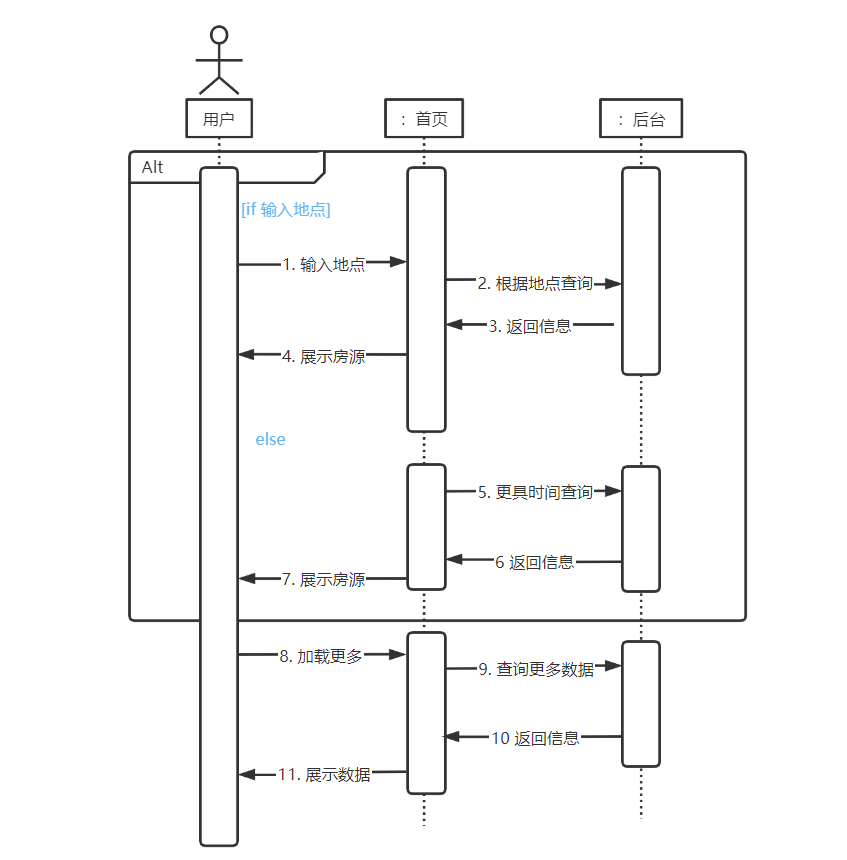
\includegraphics[width=0.7\textwidth]{ch4/viewHouseSD.png}
    \caption{浏览救助房源顺序图}\label{fig:viewHouseSD}
    \vspace{\baselineskip} % 表示图与正文空一行
\end{figure}
\subsection{活动图}
浏览救助房源的活动图如图~\ref{fig:viewHouseAD}~所示。
\begin{figure}[htbp]
    \centering
    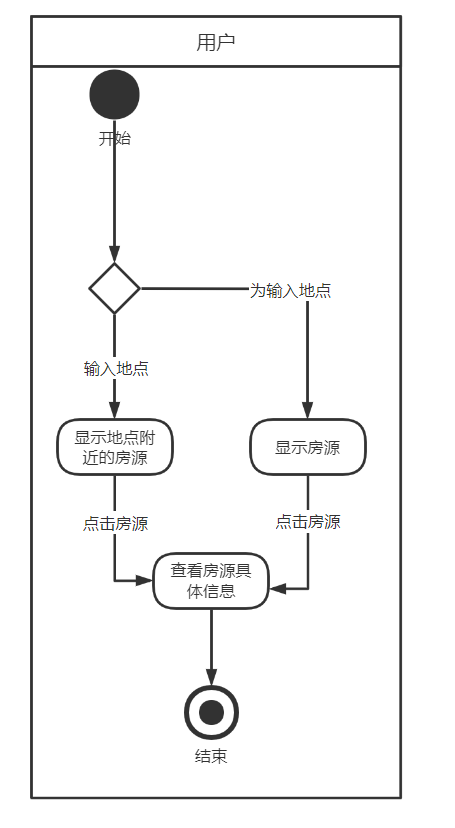
\includegraphics[width=0.6\textwidth]{ch4/viewHouseAD.png}
    \caption{浏览救助房源活动图}\label{fig:viewHouseAD}
    \vspace{\baselineskip} % 表示图与正文空一行
\end{figure}
\newpage
\subsection{状态机图}
浏览救助房源的活动图如图~\ref{fig:viewHouseFSM}~所示。
\begin{figure}[htbp]
    \centering
    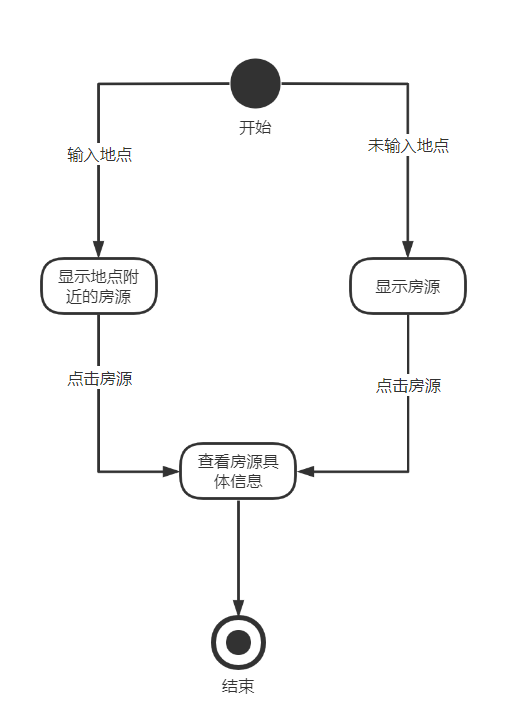
\includegraphics[width=0.6\textwidth]{ch4/viewHouseFSM.png}
    \caption{浏览救助房源状态机图}\label{fig:viewHouseFSM}
    \vspace{\baselineskip} % 表示图与正文空一行
\end{figure}

% 查询救助房源流程

\section{查询救助房源流程}
房主在发布房源信息的时候会根据给出一定的条件,比如人数显示,是否允许带宠物,语言要求,医疗救助等等。用户在查询的时候,可以通过输入地点来查询附近的救助房源信息。
在此基础上,可以通过筛选条件来筛选出符合自己的需求的救助房源信息。
\subsection{顺序图}
查询救助房源的顺序图如图~\ref{fig:conditionQuerySD}~所示。
\begin{figure}[htbp]
    \centering
    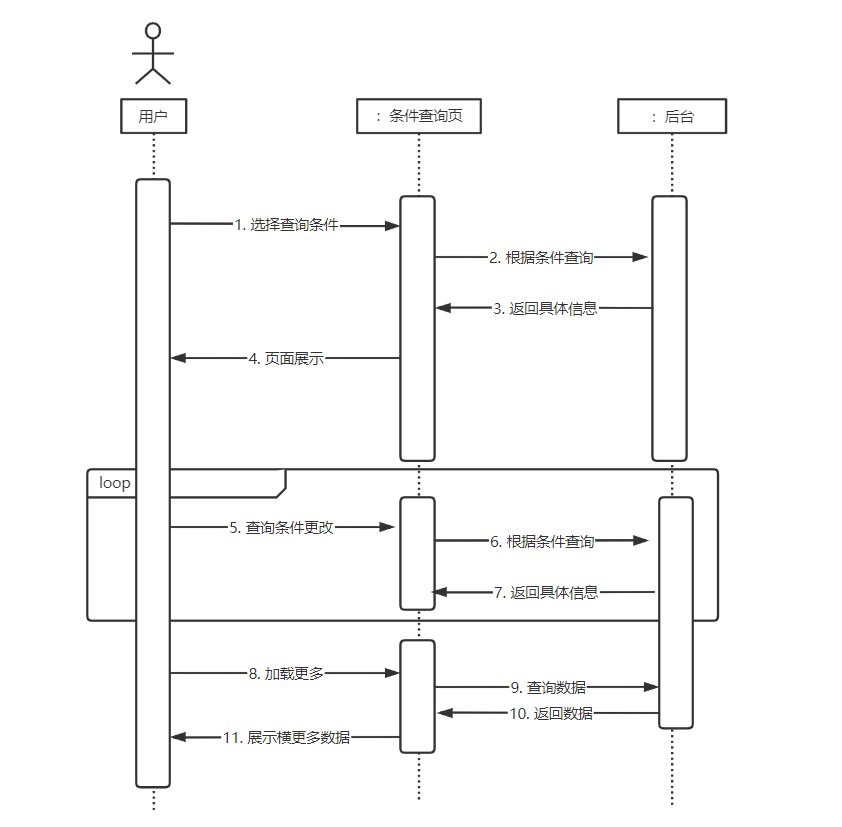
\includegraphics[width=0.8\textwidth]{ch4/conditionQuerySD.png}
    \caption{查询救助房源顺序图}\label{fig:conditionQuerySD}
    \vspace{\baselineskip} % 表示图与正文空一行
\end{figure}
\newpage
\subsection{活动图}
查询救助房源的顺序图如图~\ref{fig:conditionQueryAD}~所示。
\begin{figure}[htbp]
    \centering
    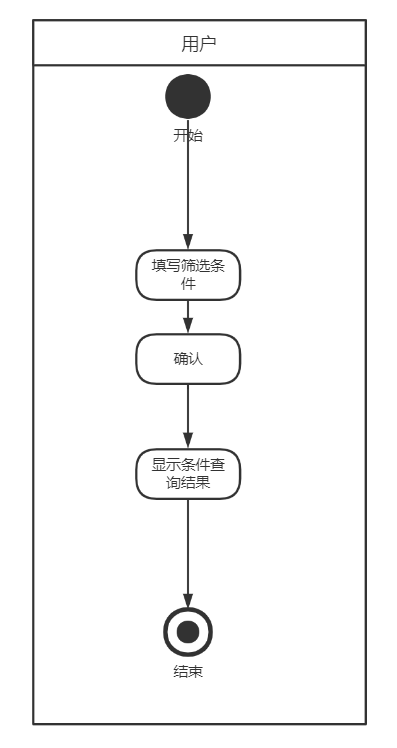
\includegraphics[width=0.6\textwidth]{ch4/conditionQueryAD.png}
    \caption{查询救助房源活动图}\label{fig:conditionQueryAD}
    \vspace{\baselineskip} % 表示图与正文空一行
\end{figure}
\newpage
\subsection{状态机图}
查询救助房源的顺序图如图~\ref{fig:conditionQueryFSM}~所示。
\begin{figure}[htbp]
    \centering
    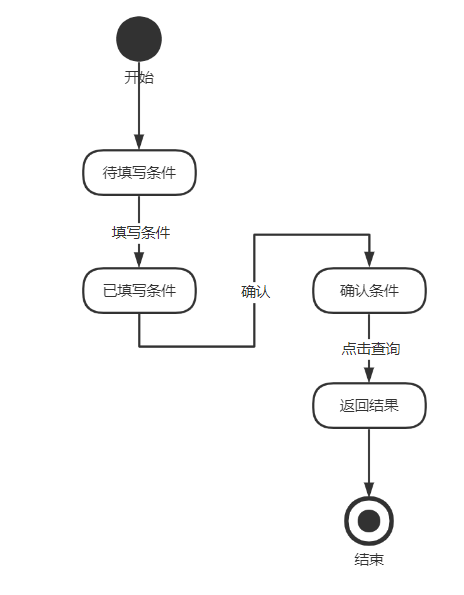
\includegraphics[width=0.6\textwidth]{ch4/conditionQueryFSM.png}
    \caption{查询救助房源状态机图}\label{fig:conditionQueryFSM}
    \vspace{\baselineskip} % 表示图与正文空一行
\end{figure}

% 举报流程 

\section{举报流程}
\subsection{顺序图}
对于举报功能,举报者可以是难民,编辑员和房主,被举报者是编译员和房主。举报房主默认举报内容是房源信息,举报编辑员默认举报内容是发布的新闻。
举报功能必须要用户登录才能使用。举报之后,举报信息的状态是待定,管理员审核之后如果同意,管理员会删除被举报者的相关发布,并且通知被举报者和举报者。
如果举报不通过,管理员会通知举报者说明理由,举报者可以选择修改举报之后再次举报或者选择放弃举报。
举报流程的顺序图如图~\ref{fig:jubaoSD}~所示。
\begin{figure}[htbp]
    \centering
    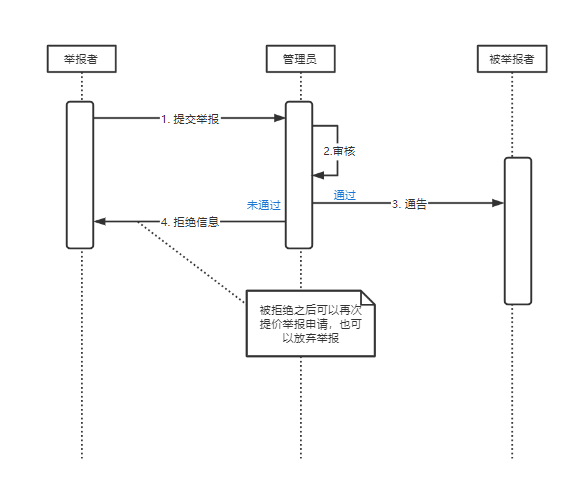
\includegraphics[width=\textwidth]{ch4/jubaoSD.png}
    \caption{举报顺序图}\label{fig:jubaoSD}
    \vspace{\baselineskip} % 表示图与正文空一行
\end{figure}
\subsection{活动图}
举报流程的活动图如图~\ref{fig:jubaoAD}~所示。
\begin{figure}[htbp]
    \centering
    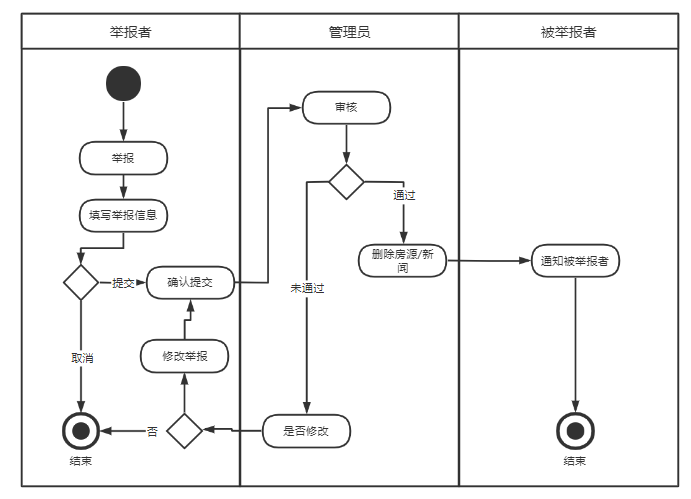
\includegraphics[width=0.8\textwidth]{ch4/jubaoAD.png}
    \caption{举报活动图}\label{fig:jubaoAD}
    \vspace{\baselineskip} % 表示图与正文空一行
\end{figure}
\subsection{状态机图}
举报流程的状态机图如图~\ref{fig:jubaoFSM}~所示。
\begin{figure}[htbp]
    \centering
    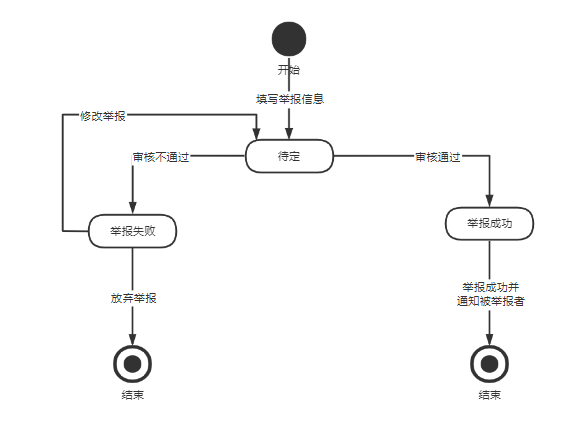
\includegraphics[width=0.8\textwidth]{ch4/jubaoFSM.png}
    \caption{举报状态机图}\label{fig:jubaoFSM}
    \vspace{\baselineskip} % 表示图与正文空一行
\end{figure}

\section{查看新闻}
\subsection{顺序图}
查看新闻的顺序图如图~\ref{fig:newsSD}~所示。
新闻板块是用户可以产看新闻的板块,主要用户推送战时新闻,包括但不限于领导人的谈判结果,国际社会的援助等。在此基础上,用户可以举报新闻,具体流程见上一节。
\begin{figure}[htbp]
    \centering
    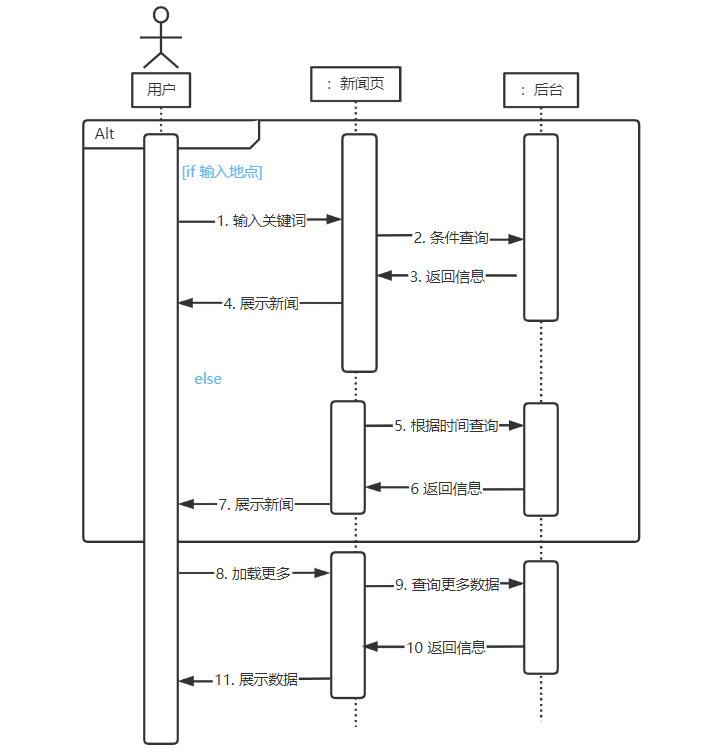
\includegraphics[width=\textwidth]{ch4/newsSD.png}
    \caption{查看新闻顺序图}\label{fig:newsSD}
    \vspace{\baselineskip} % 表示图与正文空一行
\end{figure}
\subsection{活动图}
查看新闻的活动图如图~\ref{fig:newsAD}~所示。
\begin{figure}[htbp]
    \centering
    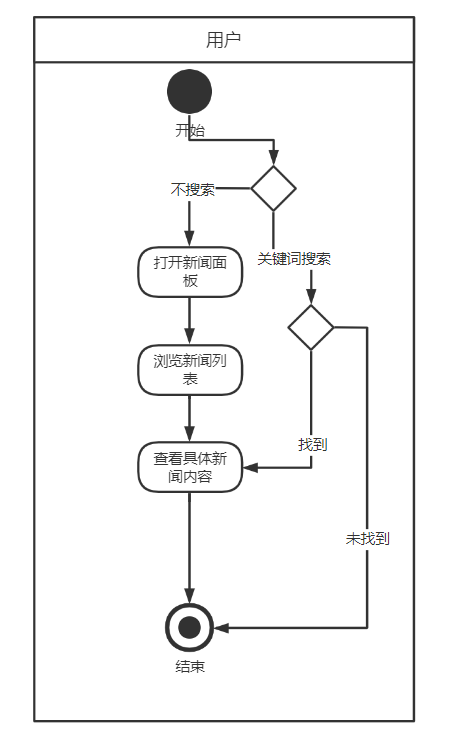
\includegraphics[width=.6\textwidth]{ch4/newsAD.png}
    \caption{查看新闻活动图}\label{fig:newsAD}
    \vspace{\baselineskip} % 表示图与正文空一行
\end{figure}
\subsection{状态机图}
查看新闻的状态机图如图~\ref{fig:newsFSM}~所示。
\begin{figure}[htbp]
    \centering
    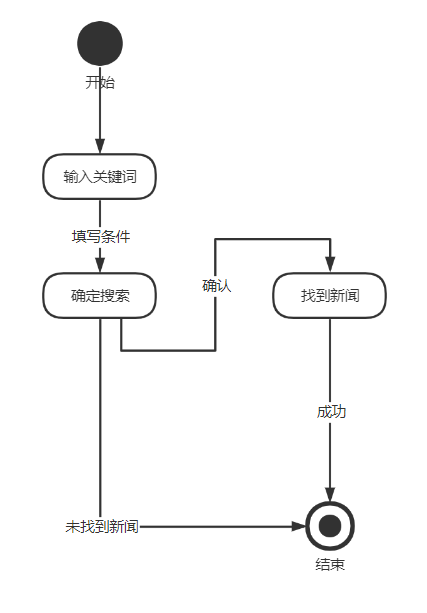
\includegraphics[width=.6\textwidth]{ch4/newsFSM.png}
    \caption{查看新闻状态机图}\label{fig:newsFSM}
    \vspace{\baselineskip} % 表示图与正文空一行
\end{figure}

\section{查看救援地图流程}
在这个板块,用户可以查看自己附近的救援信息,当然也可以输入地点来查看输入地点的附近的救助点。在地图上会显示出相对应的图标,用户点击对应的图标能够展示出救助的一些基本信息供用户参考。
也可以根据显示的结果直接在条件查询板块,将想要查询的板块输入作为条件。
\subsection{顺序图}
查看救援地图的顺序图如图~\ref{fig:mapSD}~所示。
\begin{figure}[htbp]
    \centering
    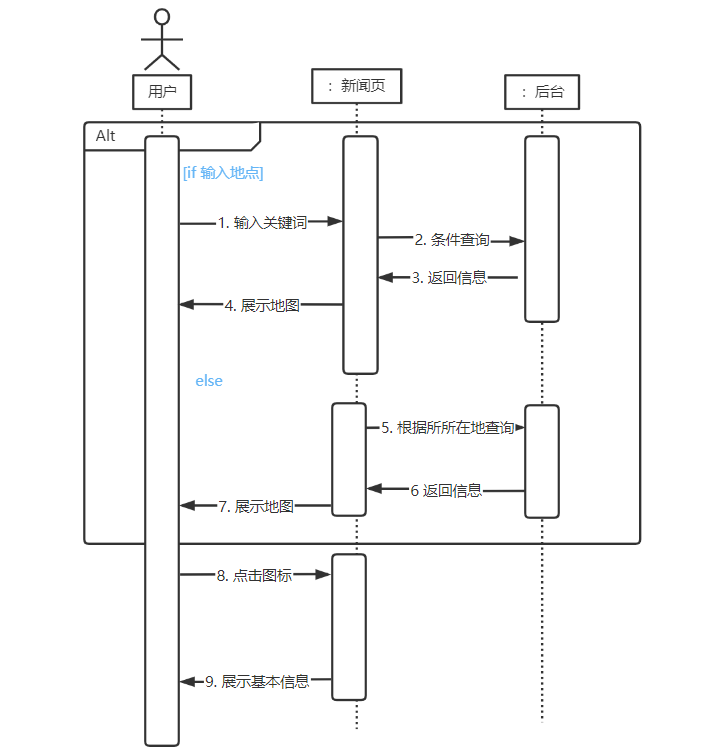
\includegraphics[width=0.8\textwidth]{ch4/mapSD.png}
    \caption{查看救援地图顺序图}\label{fig:mapSD}
    \vspace{\baselineskip} % 表示图与正文空一行
\end{figure}
\subsection{活动图}
查看救援地图的活动图如图~\ref{fig:mapAD}~所示。
\begin{figure}[htbp]
    \centering
    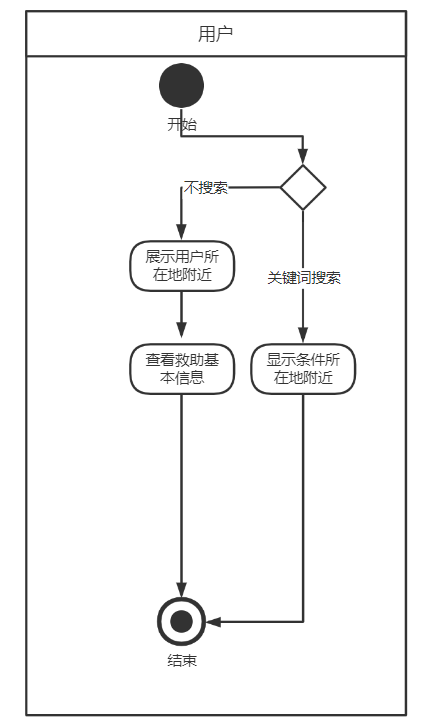
\includegraphics[width=.6\textwidth]{ch4/mapAD.png}
    \caption{查看救援地图顺序图}\label{fig:mapAD}
    \vspace{\baselineskip} % 表示图与正文空一行
\end{figure}
\subsection{状态机图}
查看救援地图的状态机图如图~\ref{fig:mapFSM}~所示。
\begin{figure}[htbp]
    \centering
    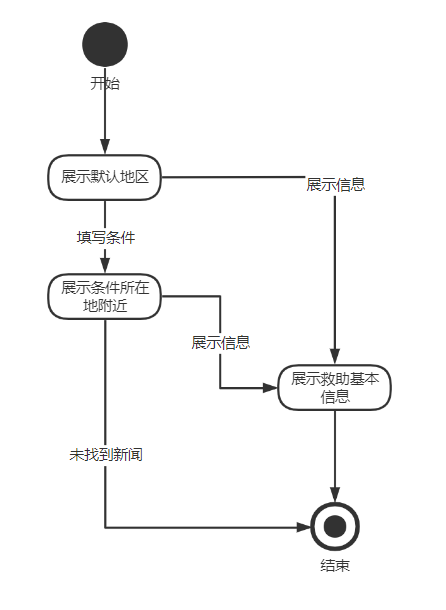
\includegraphics[width=.6\textwidth]{ch4/mapFSM.png}
    \caption{查看救援地图顺序图}\label{fig:mapFSM}
    \vspace{\baselineskip} % 表示图与正文空一行
\end{figure}

\section{登录流程}
用户登录市一切需要对数据库有更改的操作的基础。登录之后,可以实现举报功能,也是身份认证的基础。
\subsection{顺序图}
登录的顺序图如图~\ref{fig:loginSD}~所示。
\begin{figure}[htbp]
    \centering
    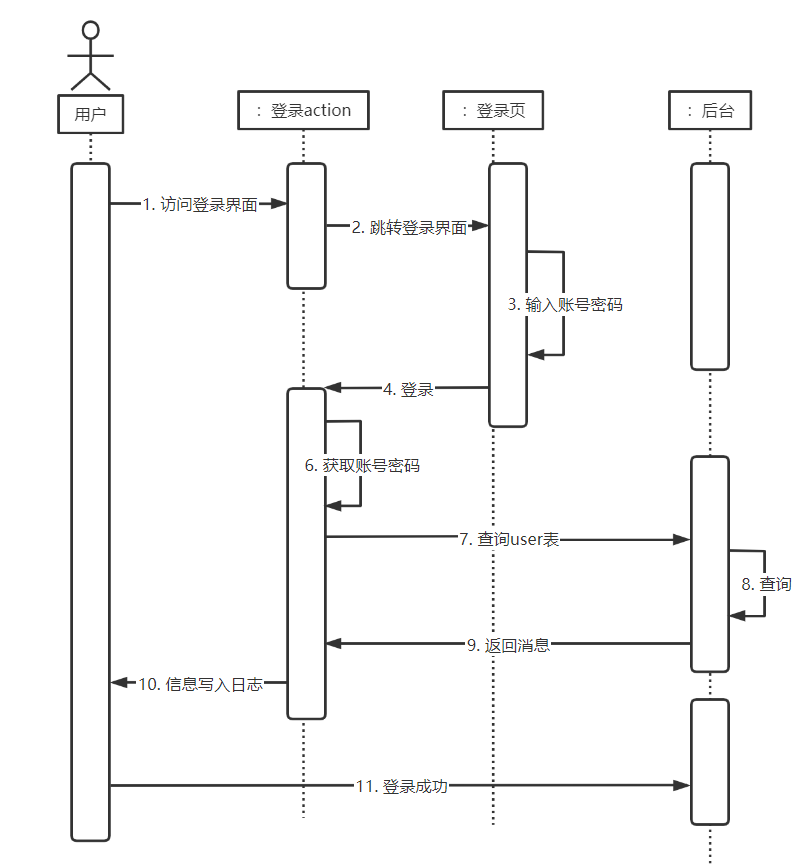
\includegraphics[width=\textwidth]{ch4/loginSD.png}
    \caption{登录顺序图}\label{fig:loginSD}
    \vspace{\baselineskip} % 表示图与正文空一行
\end{figure}
\subsection{活动图}
登录的活动图如图~\ref{fig:loginAD}~所示。
\begin{figure}[htbp]
    \centering
    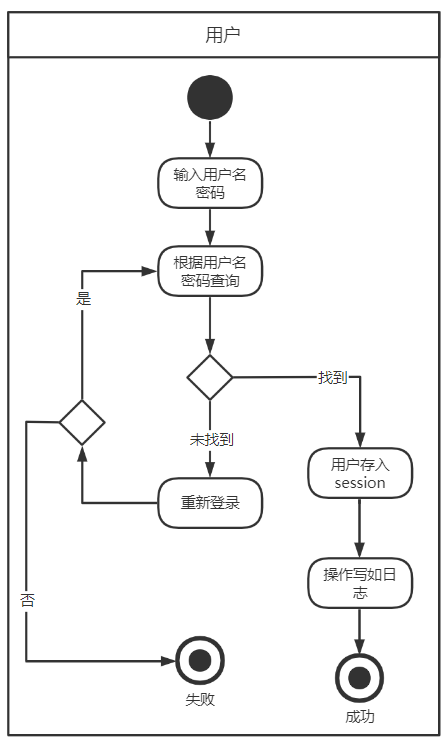
\includegraphics[width=.6\textwidth]{ch4/loginAD.png}
    \caption{登录顺序图}\label{fig:loginAD}
    \vspace{\baselineskip} % 表示图与正文空一行
\end{figure}
\subsection{状态机图}
登录的状态机图如图~\ref{fig:loginFSM}~所示。
\begin{figure}[htbp]
    \centering
    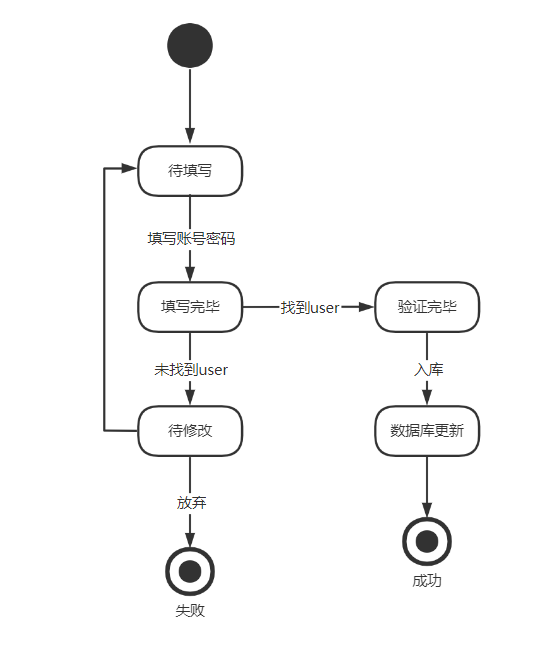
\includegraphics[width=.6\textwidth]{ch4/loginFSM.png}
    \caption{登录顺序图}\label{fig:loginFSM}
    \vspace{\baselineskip} % 表示图与正文空一行
\end{figure}

\section{身份认证流程}
\subsection{顺序图}
房主在登录之后,需要身份认证之后才能发布房源。
身份认证的顺序图如图~\ref{fig:idSD}~所示。
\begin{figure}[htbp]
    \centering
    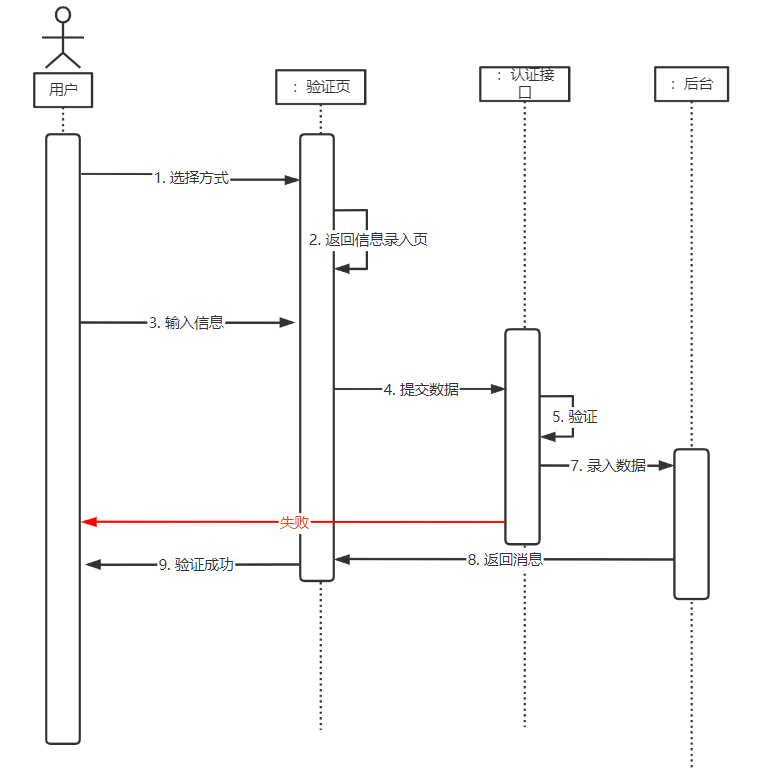
\includegraphics[width=\textwidth]{ch4/idSD.png}
    \caption{身份认证顺序图}\label{fig:idSD}
    \vspace{\baselineskip} % 表示图与正文空一行
\end{figure}
\subsection{活动图}
身份认证的活动图如图~\ref{fig:idAD}~所示。
\begin{figure}[htbp]
    \centering
    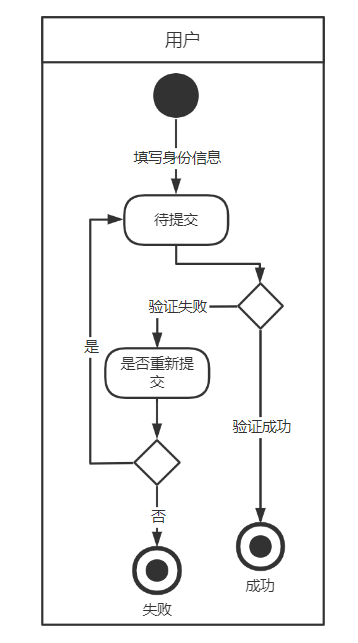
\includegraphics[width=.6\textwidth]{ch4/idAD.png}
    \caption{身份认证活动图}\label{fig:idAD}
    \vspace{\baselineskip} % 表示图与正文空一行
\end{figure}
\subsection{状态机图}
身份认证的状态机图如图~\ref{fig:idFSM}~所示。
\begin{figure}[htbp]
    \centering
    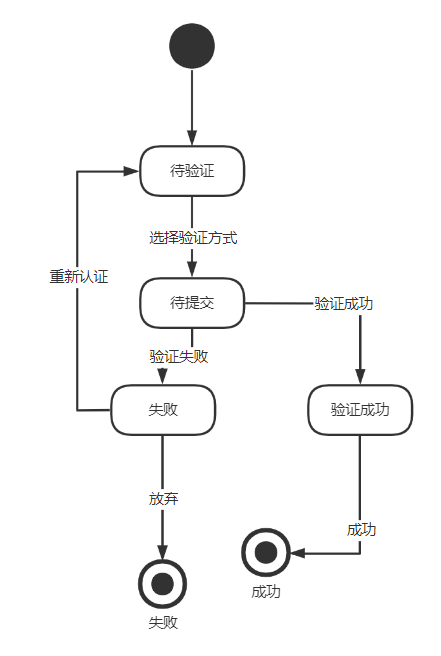
\includegraphics[width=.6\textwidth]{ch4/idFSM.png}
    \caption{身份认证状态机图}\label{fig:idFSM}
    \vspace{\baselineskip} % 表示图与正文空一行
\end{figure}

\section{添加房源/新闻信息流程}
房主在身份认证之后可以发布房源信息,在发布的时候,系统会做一些基本校验。不通过需要更改。
\subsection{顺序图}
添加房源/新闻的顺序图如图~\ref{fig:addhouseSD}~所示。
\begin{figure}[htbp]
    \centering
    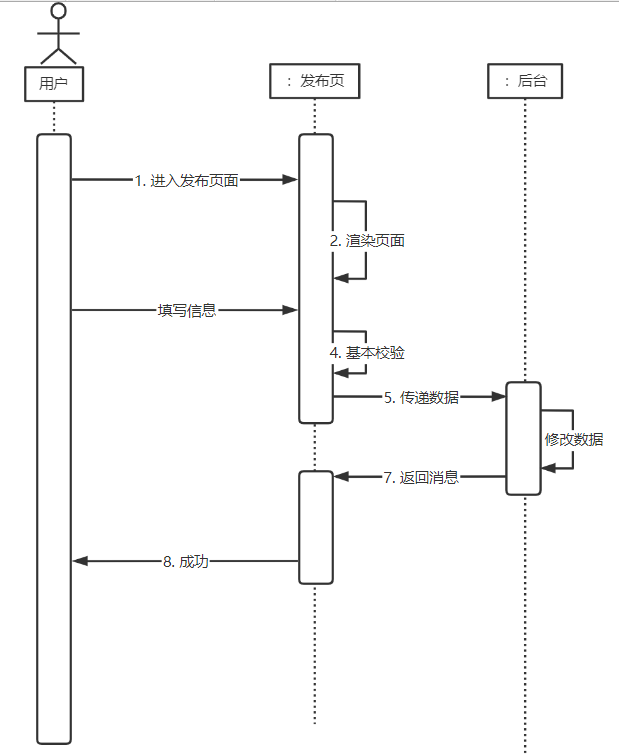
\includegraphics[width=.6\textwidth]{ch4/addhouseSD.png}
    \caption{添加房源/新闻顺序图}\label{fig:addhouseSD}
    \vspace{\baselineskip} % 表示图与正文空一行
\end{figure}
\subsection{活动图}
添加房源/新闻的活动图如图~\ref{fig:addhouseAD}~所示。
\begin{figure}[htbp]
    \centering
    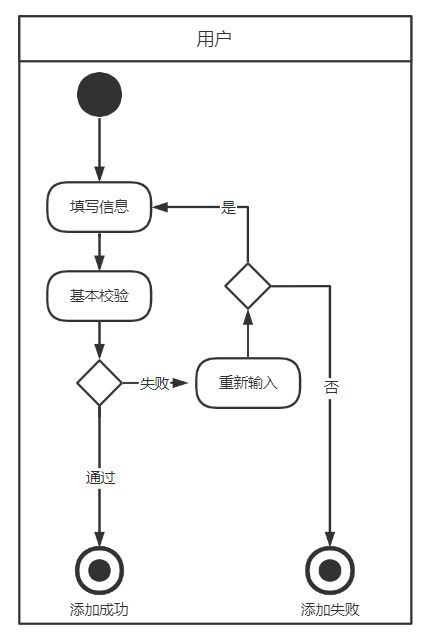
\includegraphics[width=.6\textwidth]{ch4/addhouseAD.png}
    \caption{添加房源/新闻活动图}\label{fig:addhouseAD}
    \vspace{\baselineskip} % 表示图与正文空一行
\end{figure}
\subsection{状态机图}
添加房源/新闻的状态机图如图~\ref{fig:addhouseFSM}~所示。
\begin{figure}[htbp]
    \centering
    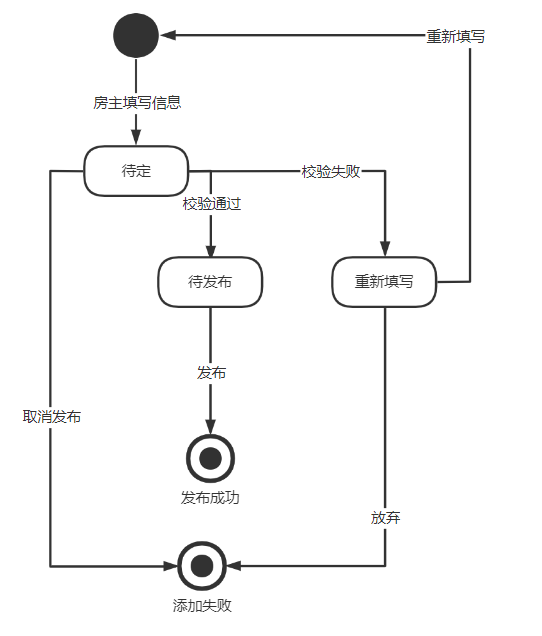
\includegraphics[width=.6\textwidth]{ch4/addhouseFSM.png}
    \caption{添加房源/新闻状态机图}\label{fig:addhouseFSM}
    \vspace{\baselineskip} % 表示图与正文空一行
\end{figure}

\section{修改房源/新闻信息流程}
用户在被举报之后可以修改自己的房源,或者自己主动更改。
\subsection{顺序图}
修改房源/新闻的顺序图如图~\ref{fig:alterhouseSD}~所示。
\begin{figure}[htbp]
    \centering
    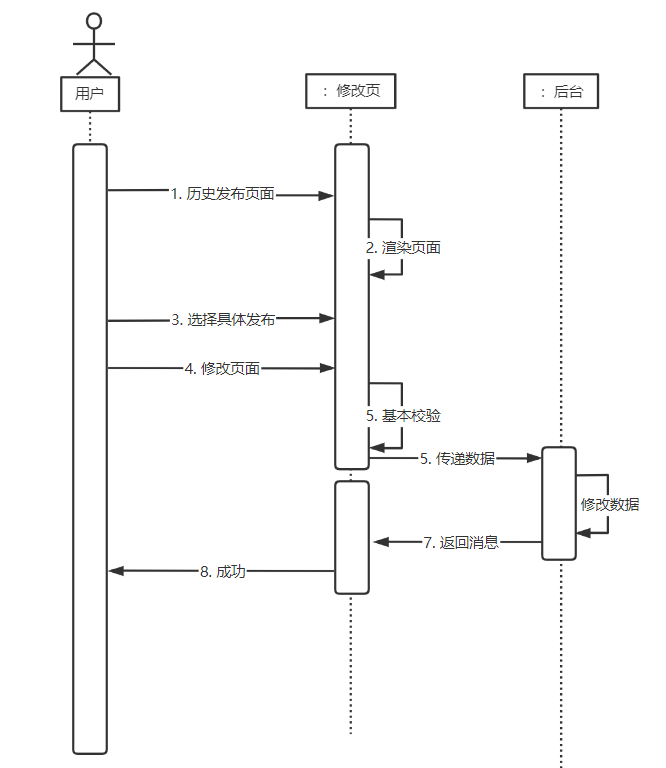
\includegraphics[width=.8\textwidth]{ch4/alterhouseSD.png}
    \caption{修改房源/新闻顺序图}\label{fig:alterhouseSD}
    \vspace{\baselineskip} % 表示图与正文空一行
\end{figure}
\subsection{活动图}
修改房源/新闻的活动图如图~\ref{fig:alterhouseAD}~所示。
\begin{figure}[htbp]
    \centering
    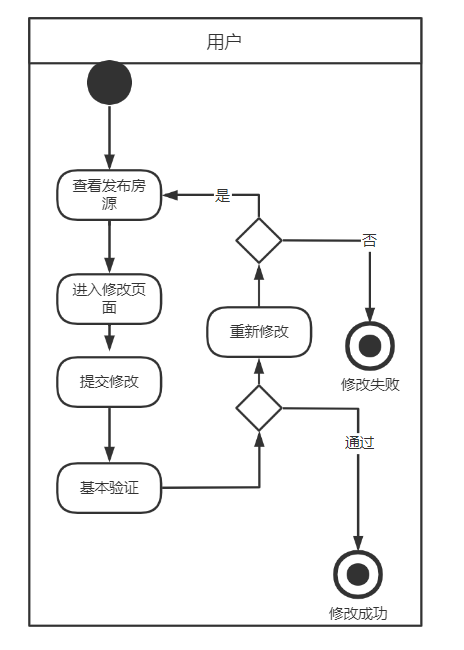
\includegraphics[width=.6\textwidth]{ch4/alterhouseAD.png}
    \caption{修改房源/新闻活动图}\label{fig:alterhouseAD}
    \vspace{\baselineskip} % 表示图与正文空一行
\end{figure}
\subsection{状态机图}
修改房源/新闻的状态机图如图~\ref{fig:alterhouseFSM}~所示。
\begin{figure}[htbp]
    \centering
    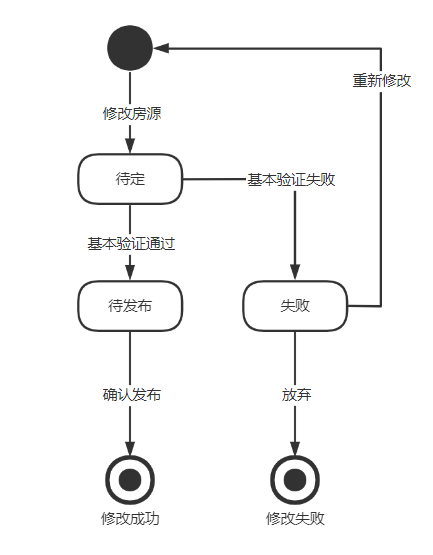
\includegraphics[width=.6\textwidth]{ch4/alterhouseFSM.png}
    \caption{修改房源/新闻状态机图}\label{fig:alterhouseFSM}
    \vspace{\baselineskip} % 表示图与正文空一行
\end{figure}

\section{删除房源/新闻信息流程}
用户可以自主删除发布的房源信息和
\subsection{顺序图}
删除房源/新闻的顺序图如图~\ref{fig:deleteSD}~所示。
\begin{figure}[htbp]
    \centering
    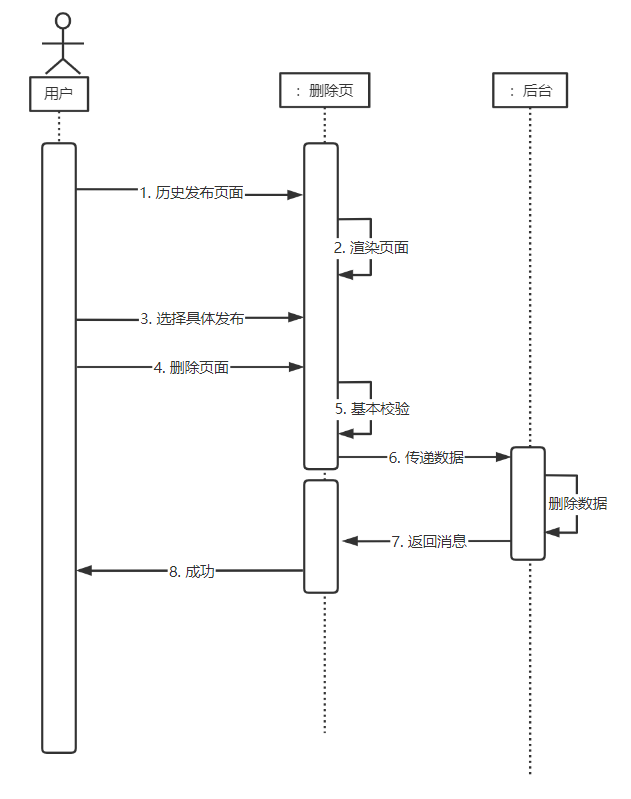
\includegraphics[width=.8\textwidth]{ch4/deleteSD.png}
    \caption{删除房源/新闻顺序图}\label{fig:deleteSD}
    \vspace{\baselineskip} % 表示图与正文空一行
\end{figure}
\subsection{活动图}
删除房源/新闻的活动图如图~\ref{fig:deleteAD}~所示。
\begin{figure}[htbp]
    \centering
    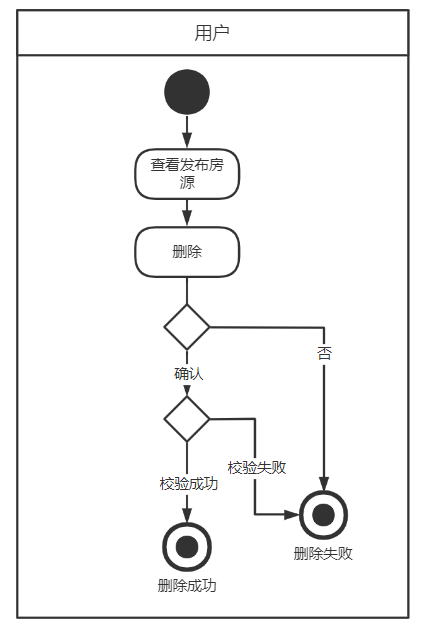
\includegraphics[width=.6\textwidth]{ch4/deleteAD.png}
    \caption{删除房源/新闻活动图}\label{fig:deleteAD}
    \vspace{\baselineskip} % 表示图与正文空一行
\end{figure}
\subsection{状态机图}
删除房源/新闻的状态机图如图~\ref{fig:deleteFSM}~所示。
\begin{figure}[htbp]
    \centering
    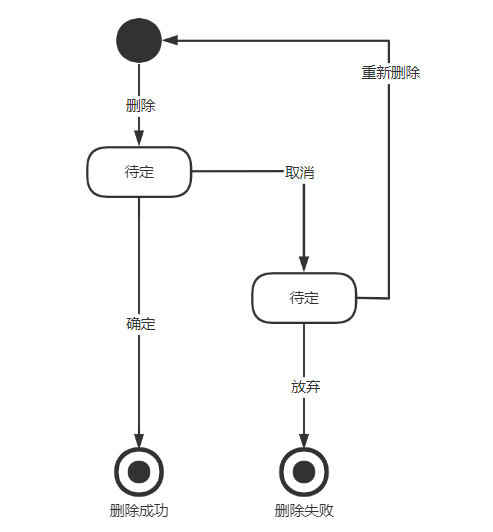
\includegraphics[width=.6\textwidth]{ch4/deleteFSM.png}
    \caption{删除房源/新闻状态机图}\label{fig:deleteFSM}
    \vspace{\baselineskip} % 表示图与正文空一行
\end{figure}

\section{修改菜单项流程}
管理员有权限来改变菜单项,但是不是所有的时候都可以修改,如果当前有用户正在对于菜单项中对应的页面进行读写操作,就不能进行更新操作。
\subsection{顺序图}
修改菜单项的顺序图如图~\ref{fig:menuSD}~所示。
\begin{figure}[htbp]
    \centering
    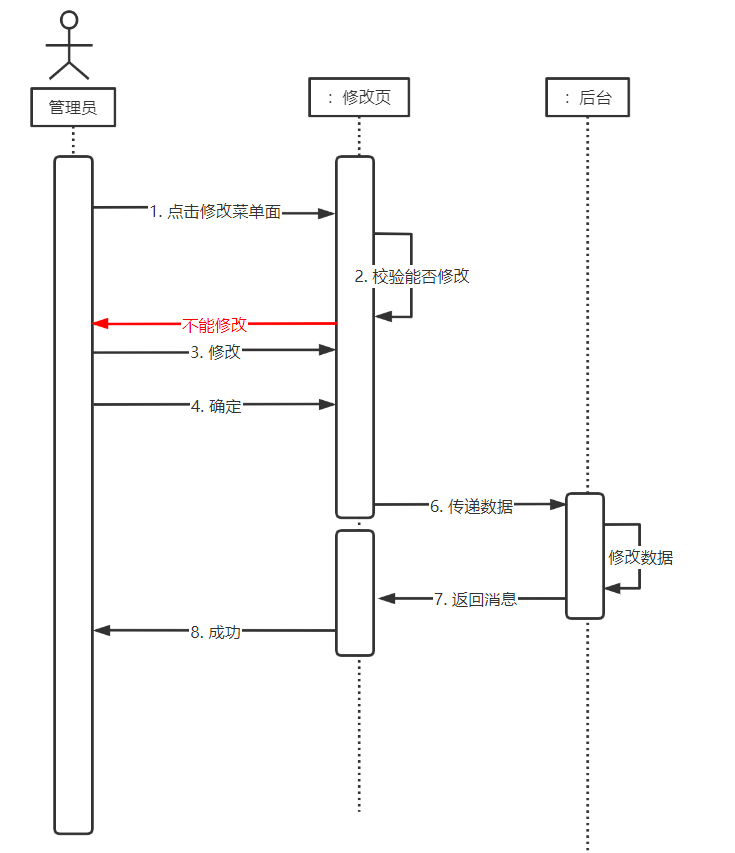
\includegraphics[width=.8\textwidth]{ch4/menuSD.png}
    \caption{修改菜单项顺序图}\label{fig:menuSD}
    \vspace{\baselineskip} % 表示图与正文空一行
\end{figure}
\subsection{活动图}
修改菜单项的活动图如图~\ref{fig:menuAD}~所示。
\begin{figure}[htbp]
    \centering
    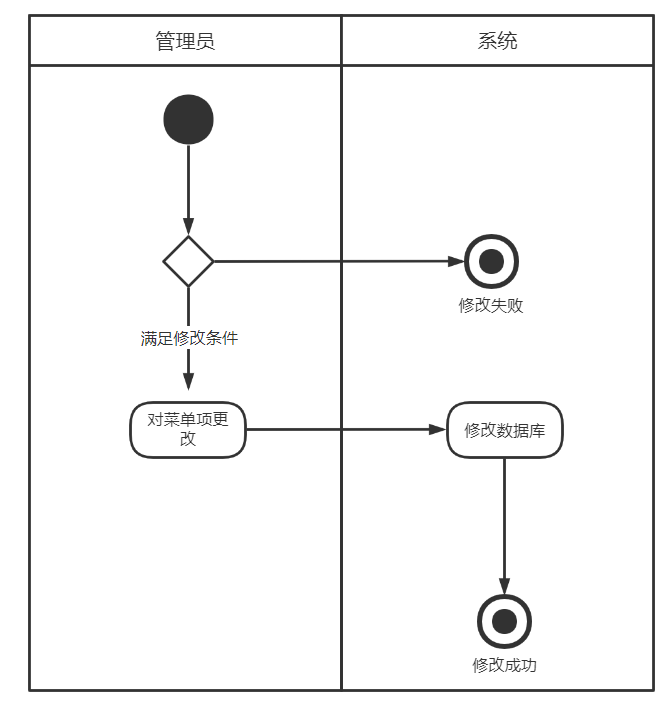
\includegraphics[width=.6\textwidth]{ch4/menuAD.png}
    \caption{修改菜单项活动图}\label{fig:menuAD}
    \vspace{\baselineskip} % 表示图与正文空一行
\end{figure}
\subsection{状态机图}
修改菜单项的状态机图如图~\ref{fig:menuFSM}~所示。
\begin{figure}[htbp]
    \centering
    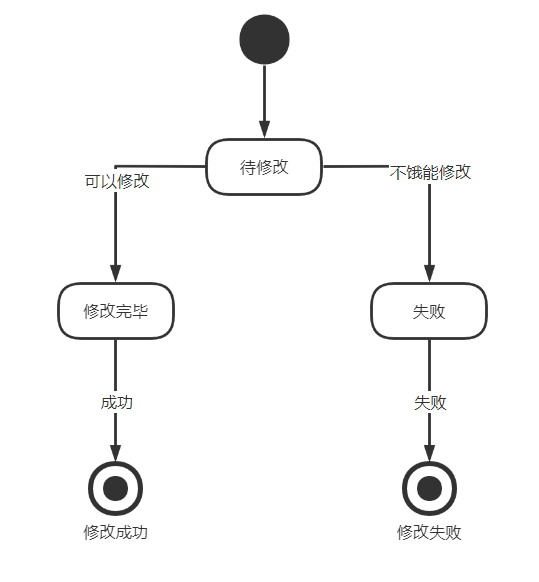
\includegraphics[width=.6\textwidth]{ch4/menuFSM.png}
    \caption{修改菜单项状态机图}\label{fig:menuFSM}
    \vspace{\baselineskip} % 表示图与正文空一行
\end{figure}

\section{管理角色权限流程}

\subsection{顺序图}
管理角色权限的顺序图如图~\ref{fig:roleauthoritySD}~所示。
\begin{figure}[htbp]
    \centering
    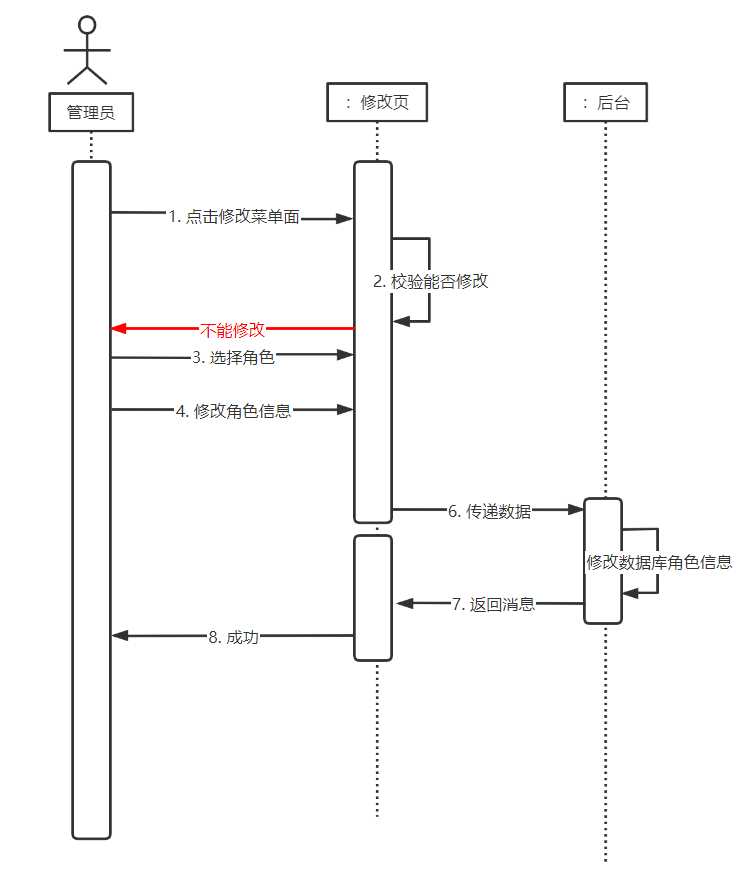
\includegraphics[width=.8\textwidth]{ch4/roleauthoritySD.png}
    \caption{管理角色权限顺序图}\label{fig:roleauthoritySD}
    \vspace{\baselineskip} % 表示图与正文空一行
\end{figure}
\subsection{活动图}
管理角色权限的活动图如图~\ref{fig:roleauthorityAD}~所示。
\begin{figure}[htbp]
    \centering
    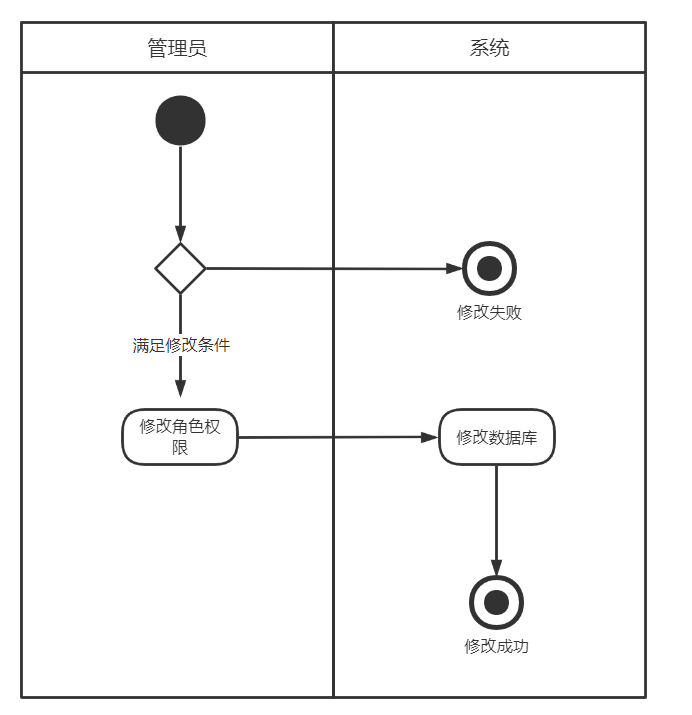
\includegraphics[width=.6\textwidth]{ch4/roleauthorityAD.png}
    \caption{管理角色权限活动图}\label{fig:roleauthorityAD}
    \vspace{\baselineskip} % 表示图与正文空一行
\end{figure}
\subsection{状态机图}
管理角色权限的状态机图如图~\ref{fig:roleauthorityFSM}~所示。
\begin{figure}[htbp]
    \centering
    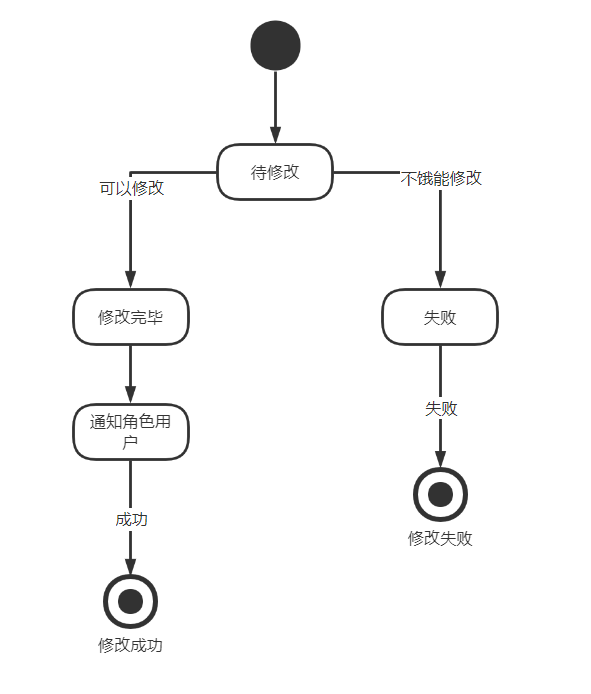
\includegraphics[width=.6\textwidth]{ch4/roleauthorityFSM.png}
    \caption{管理角色权限状态机图}\label{fig:roleauthorityFSM}
    \vspace{\baselineskip} % 表示图与正文空一行
\end{figure}

\section{管理用户权限流程}
管理员可以对于指定的特定用户进行权限管理,比如对于被举报次数过多的房主可以撤销发布救助房源的权限。
\subsection{顺序图}
管理用户权限的顺序图如图~\ref{fig:userauthoritySD}~所示。
\begin{figure}[htbp]
    \centering
    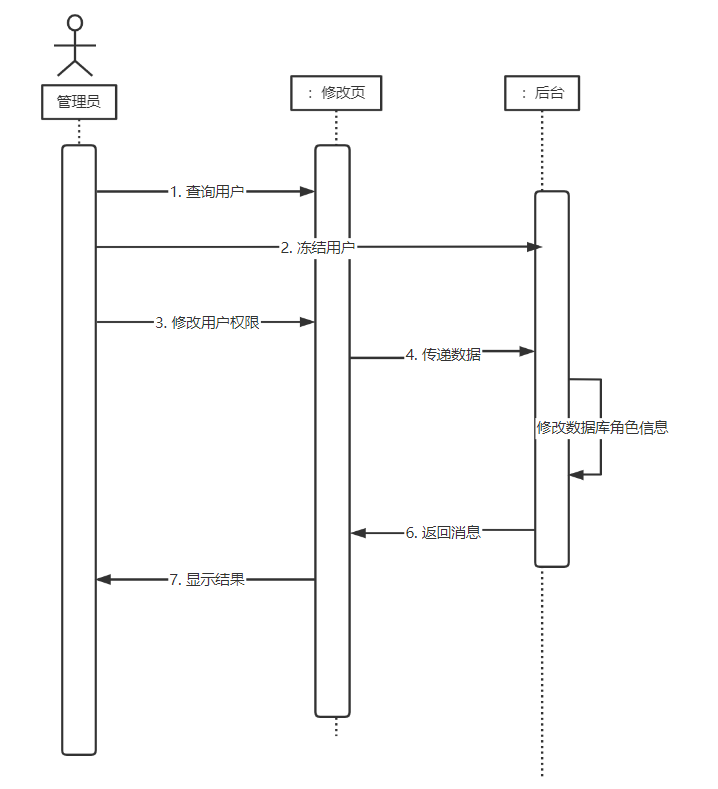
\includegraphics[width=.8\textwidth]{ch4/userauthoritySD.png}
    \caption{管理用户权限顺序图}\label{fig:userauthoritySD}
    \vspace{\baselineskip} % 表示图与正文空一行
\end{figure}
\subsection{活动图}
管理用户权限的活动图如图~\ref{fig:userauthorityAD}~所示。
\begin{figure}[htbp]
    \centering
    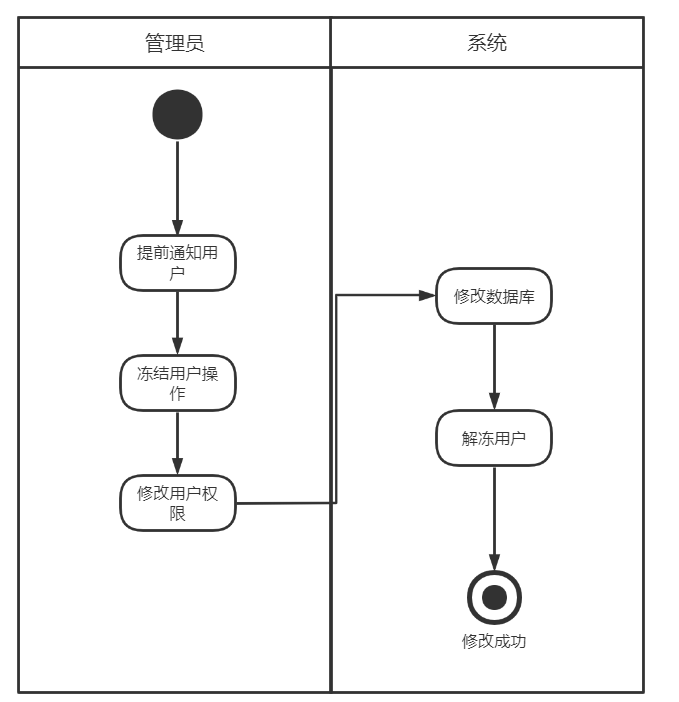
\includegraphics[width=.6\textwidth]{ch4/userauthorityAD.png}
    \caption{管理用户权限活动图}\label{fig:userauthorityAD}
    \vspace{\baselineskip} % 表示图与正文空一行
\end{figure}
\subsection{状态机图}
管理用户权限的状态机图如图~\ref{fig:userauthorityFSM}~所示。
\begin{figure}[htbp]
    \centering
    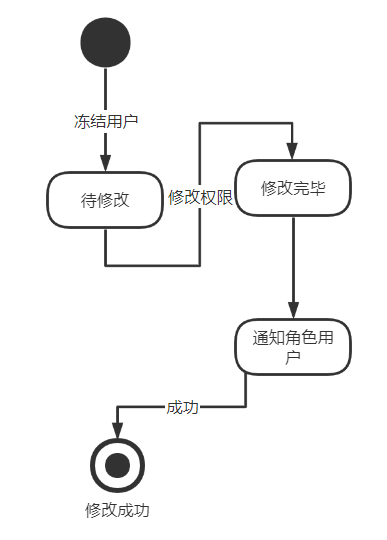
\includegraphics[width=.6\textwidth]{ch4/userauthorityFSM.png}
    \caption{管理用户权限状态机图}\label{fig:userauthorityFSM}
    \vspace{\baselineskip} % 表示图与正文空一行
\end{figure}

\section{管理用户流程}

\subsection{顺序图}
用户管理的顺序图如图~\ref{fig:usercontrolSD}~所示。
\begin{figure}[htbp]
    \centering
    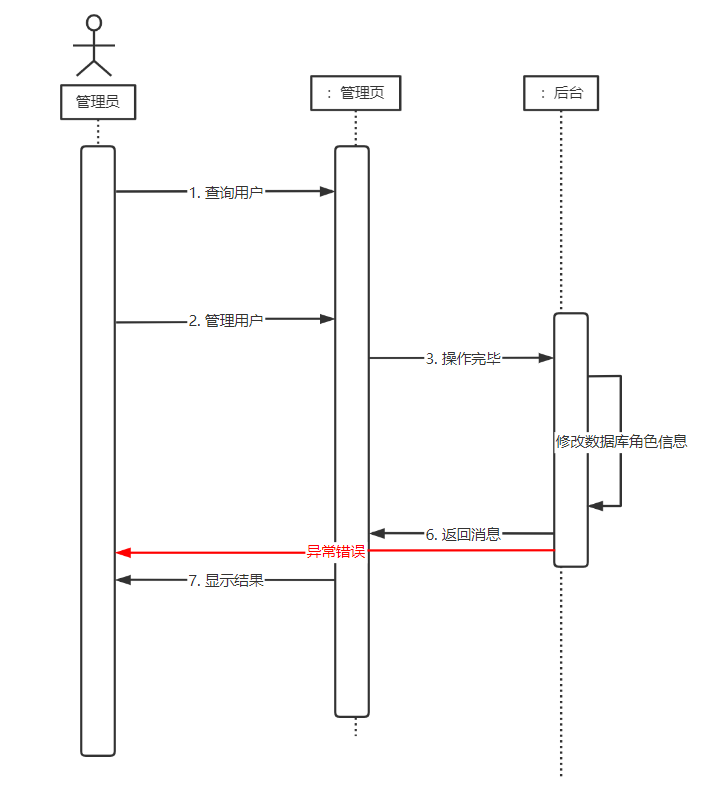
\includegraphics[width=.8\textwidth]{ch4/usercontrolSD.png}
    \caption{管理用户权限顺序图}\label{fig:usercontrolSD}
    \vspace{\baselineskip} % 表示图与正文空一行
\end{figure}
\subsection{活动图}
用户管理的活动图如图~\ref{fig:usercontrolAD}~所示。
\begin{figure}[htbp]
    \centering
    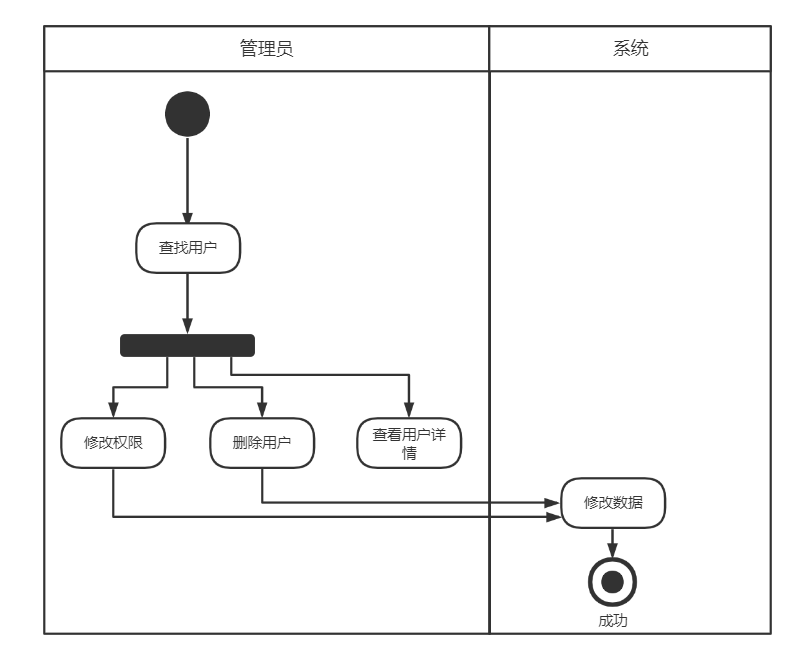
\includegraphics[width=.6\textwidth]{ch4/usercontrolAD.png}
    \caption{管理用户权限活动图}\label{fig:usercontrolAD}
    \vspace{\baselineskip} % 表示图与正文空一行
\end{figure}
\subsection{状态机图}
用户管理的状态机图如图~\ref{fig:usercontrolFSM}~所示。
\begin{figure}[htbp]
    \centering
    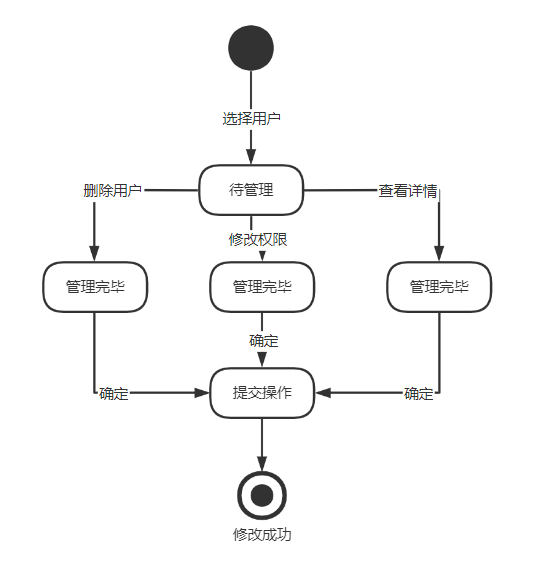
\includegraphics[width=.6\textwidth]{ch4/usercontrolFSM.png}
    \caption{管理用户权限状态机图}\label{fig:usercontrolFSM}
    \vspace{\baselineskip} % 表示图与正文空一行
\end{figure}